\documentclass[a4paper, 12pt]{report}
% Forces PDF version 1.7
\pdfminorversion=7
% Allows writing the document in english.
\usepackage[utf8]{inputenc}
\usepackage[francais]{babel}
\usepackage[T1]{fontenc}
% Allows to use images.
\usepackage{graphicx}
% Provides hyperlinks within the document.
\usepackage{enumitem}
% Adds space between paragraphs.
\usepackage{parskip}
% Supports Text Companion fonts (necessary for gensymb).
\usepackage{textcomp}
\usepackage{array}
\usepackage{multicol}
% Better tabular
\usepackage{tabularx}
% Allows to use colors.
\usepackage{xcolor}
\usepackage[margin=4cm]{geometry}
\usepackage{varwidth}
% Euro
\usepackage{eurosym}
\usepackage{amsmath}

\usepackage{subfigure}
\usepackage[
    type={CC},
    modifier={by-nc-nd},
    version={4.0},
]{doclicense}

\usepackage[colorlinks=true,urlcolor=black,linkcolor=black]{hyperref}
% New columns types
% Left
\newcolumntype{L}{>{\raggedright\arraybackslash}X}
% Center
\newcolumntype{C}{>{\centering\arraybackslash}X}
% Right
\newcolumntype{R}{>{\raggedleft\arraybackslash}X}

% Add more space before and after table
\newenvironment{centerspace}{\setlength{\topsep}{1ex}\center}{\endcenter}
% Sets the color of gray.
\newcommand{\gray}{\rowcolor[gray]{.90}}
% Allows to draw lines.
\newcommand{\HRule}{\rule{\linewidth}{0.5mm}}
% Uses the arabic numerals for sections.
\renewcommand{\thesection}{\arabic{section}}

% Width of text.
\addtolength{\textwidth}{2cm}
% Odd page left margin.
\addtolength{\oddsidemargin}{-1cm}
% Height of main text.
\addtolength{\textheight}{2cm}
% Removes indentation.
\setlength\parindent{0pt}
% Indicates overflow words.
\setlength{\overfullrule}{10pt}
% Height of items.
\setitemize{itemsep=1em}
% Adds the subsubsections in the TOC
\setcounter{tocdepth}{3}
\setcounter{secnumdepth}{3}

%%%%********************************************************************
% fancy quotes
\definecolor{quotemark}{gray}{0.7}
\makeatletter
\def\fquote{%
    \@ifnextchar[{\fquote@i}{\fquote@i[]}%]
           }%
\def\fquote@i[#1]{%
    \def\tempa{#1}%
    \@ifnextchar[{\fquote@ii}{\fquote@ii[]}%]
                 }%
\def\fquote@ii[#1]{%
    \def\tempb{#1}%
    \@ifnextchar[{\fquote@iii}{\fquote@iii[]}%]
                      }%
\def\fquote@iii[#1]{%
    \def\tempc{#1}%
    \vspace{1em}%
    \noindent%
    \begin{list}{}{%
         \setlength{\leftmargin}{0.1\textwidth}%
         \setlength{\rightmargin}{0.1\textwidth}%
                  }%
         \item[]%
         \begin{picture}(0,0)%
         \put(-15,-5){\makebox(0,0){\scalebox{3}{\textcolor{quotemark}{``}}}}%
         \end{picture}%
         \begingroup\itshape}%
 %%%%********************************************************************
 \def\endfquote{%
 \endgroup\par%
 \makebox[0pt][l]{%
 \hspace{0.8\textwidth}%
 \begin{picture}(0,0)(0,0)%
 \put(15,15){\makebox(0,0){%
 \scalebox{3}{\color{quotemark}''}}}%
 \end{picture}}%
 \ifx\tempa\empty%
 \else%
    \ifx\tempc\empty%
       \hfill\rule{100pt}{0.5pt}\\\mbox{}\hfill\tempa,\ \emph{\tempb}%
   \else%
       \hfill\rule{100pt}{0.5pt}\\\mbox{}\hfill\tempa,\ \emph{\tempb},\ \tempc%
   \fi\fi\par%
   \vspace{0.5em}%
 \end{list}%
 }%
 \makeatother

 %%%% ********************************************************************

% Starts roman numbering (trick to not numbering the first pages).
\pagenumbering{roman}

\begin{document}
\renewcommand{\bibname}{Références}
\begin{center}
  
\includegraphics[scale=0.12]{textures/logo/heh_bw.pdf}

  \vspace{1cm}

  \textsc{\LARGE Projet} \\ [0.5cm]
  \textsc{\Large Réalisation d'un site en PHP} \\ [0.5cm]

  \textsc{\large 2\up{ème} Bachelier en Informatique} \\ [0.2cm]

  \begingroup
  \fontfamily{pag} \selectfont 

  \HRule \\ [0.4cm] {
    \huge Programmation web \\ [0.2cm] 
  }
  \HRule \\ [1.3cm]
  \endgroup
  \begin{minipage}[t]{0.4 \textwidth} 
    \begin{flushleft} 
      \large \emph{Auteur:} \\ 
      Alexandre \textsc{Ducobu}
    \end{flushleft} 
  \end{minipage}
  % 
  \begin{minipage}[t]{0.4 \textwidth}
    \begin{flushright} 
      \large \emph{Enseignants :} \\ 
      Antoine \textsc{Malaise} \\
      Fabrice \textsc{Scopel}
    \end{flushright} 
  \end{minipage}

  \vspace{1cm}

  
\includegraphics[scale=0.08]{textures/logo/technical_bw.pdf}

  \vspace{0.5cm}

  Année académique 2016 - 2017
\end{center}

\thispagestyle{empty}

\newpage
\newpage
\thispagestyle{empty}
\setcounter{page}{0}
\null
\newpage
\begin{center}
  
\includegraphics[scale=0.12]{textures/logo/heh.pdf}

  \vspace{2cm}

  \textsc{\LARGE Projet ARS} \\ [0.5cm]
  \textsc{\Large Les différents systèmes d'exploitation} \\ [0.5cm]

  \textsc{\large 1er Bachelier en Informatique} \\ [0.2cm]
  \textsc{Groupe 5-8} \\

  \begingroup
  \fontfamily{pag} \selectfont 

  \HRule \\ [0.4cm] {
    \huge Architecture des Systèmes II \\ [0.2cm] 
  }
  (Laboratoire)
  \HRule \\ [1.3cm]
  \endgroup

  \begin{minipage}[t]{0.4 \textwidth} 
    \begin{flushleft} 
      \large \emph{Auteur:} \\ 
      Agozzino \textsc{Terencio} 
    \end{flushleft} 
  \end{minipage}
  % 
  \begin{minipage}[t]{0.4 \textwidth}
    \begin{flushright} 
      \large \emph{Auteur :} \\ 
      Ducobu \textsc{Alexandre} 
    \end{flushright} 
  \end{minipage}

  \vspace{0.5cm}

  \begin{minipage}[t]{0.4 \textwidth}
    \begin{center} 
      \large \emph{Enseignant:} \\ 
      Desmet \textsc{Erwin} 
    \end{center} 
  \end{minipage}

  \vspace{0.5cm}

  
\includegraphics[scale=0.08]{textures/logo/technical.pdf}

  \vspace{0.5cm}

  Année académique 2015 - 2016
\end{center}

\thispagestyle{empty}

\newpage
\newpage
\thispagestyle{empty}
\setcounter{page}{0}
\null
\newpage
\newpage
\mbox{~}
\vfill
Ce document est mis à disposition selon les termes de la licence Creative
Commons ``\href{https://creativecommons.org/licenses/by-nc-nd/4.0/}{Attribution -
Pas d'utilisation commerciale 4.0 International}''.

\begin{figure}[!h]
  \centering
  
\includegraphics[width=0.25\textwidth]
  {textures/images/license/license.eps}
\end{figure}

\thispagestyle{empty}

\newpage
\pagenumbering{arabic}
\tableofcontents
\newpage
\section{Présentation du projet}
\label{sec:presentation}


\subsection{Introduction}
\label{subsec:intro}

Dans le cadre du cours de \textbf{Gestion de projets}, il nous a été demandé de réaliser un projet au choix individuellement ou par deux. J'ai choisi de le faire seul. \\
En effet, nous avons déjà d'autres travaux de groupes. Je trouve donc qu'un travail individuel est un plus dans notre cursus scolaire. \\
Lors des deux premières séances de laboratoire, chaque groupe a rédigé une fiche descriptive du projet, avec l’enseignant, afin de baliser le travail à effectuer durant l’année.\\
Lors de ces séances, l’enseignant a validé chacun des projets.


\subsection{But}
\label{subsec:but}

Grâce à ce projet, nous allons apprendre à gérer nos projets à l'aide de différents outils spécialisés tels que \textbf{\textit{Microsoft Project}}, \textit{le diagramme de \textbf{Gantt}} et \textit{le graphique de \textbf{PERT}}.\\
Ceux-ci nous aideront dans la planification de notre projet ainsi que, pour les binômes, dans la répartition des tâches. 


\subsection{Choix du projet}
\label{subsec:choix}

Ce projet, \textit{un site web}, permettra d'apprendre les bases de la programmation en \textit{Python} et sera divisé en chapitres: les variables, les conditions, les boucles, les tableaux, etc.\\

L’apprentissage se fera en trois étapes:
\begin{enumerate}
    \item L’utilisateur découvrira le nouveau sujet par de la théorie ainsi que par un ou plusieurs exemples. Il en apprendra alors l’utilité et le fonctionnement.
    \item Entre deux parties théoriques, l’utilisateur mettra en pratique ce qu’il aura appris au travers de petits QCM.
    \item Une fois le chapitre terminé, un questionnaire (QCM, ordonnancement du code,...) sera proposé à l’utilisateur.\\
    Celui-ci sera noté sur 10 afin que l’utilisateur puisse se juger et s’améliorer.\\
    Le passage au chapitre suivant requerra une \textit{cote minimale de 7/10}.\\
\end{enumerate}

D'autre part, ce projet sera un pré-TFE.\\
À terme, il sera possible de créer facilement des cours et de s’y inscrire.\\ Il pourra être utilisé aussi bien par les écoles que par  \og \textit{les particuliers} \fg.


%%% Local Variables:
%%% mode: latex
%%% TeX-master: t
%%% End:

\newpage
\section{Base de données}
\label{sec:BD}


\subsection{Création de la base de données}
\label{sec:creation-db}

La base de données est composée de trois tables contenant toutes les données utiles au bon fonctionnement du site.\\
Il y a la table \textbf{Users} \textit{pour tout ce qui concerne les utilisateurs}, la table \textbf{Medicines}, \textit{qui concerne les médicaments} et le table \textbf{Reserves} \textit{qui contient la réserve de chaque utilisateur}.

\begin{figure}[h]
  \centering
  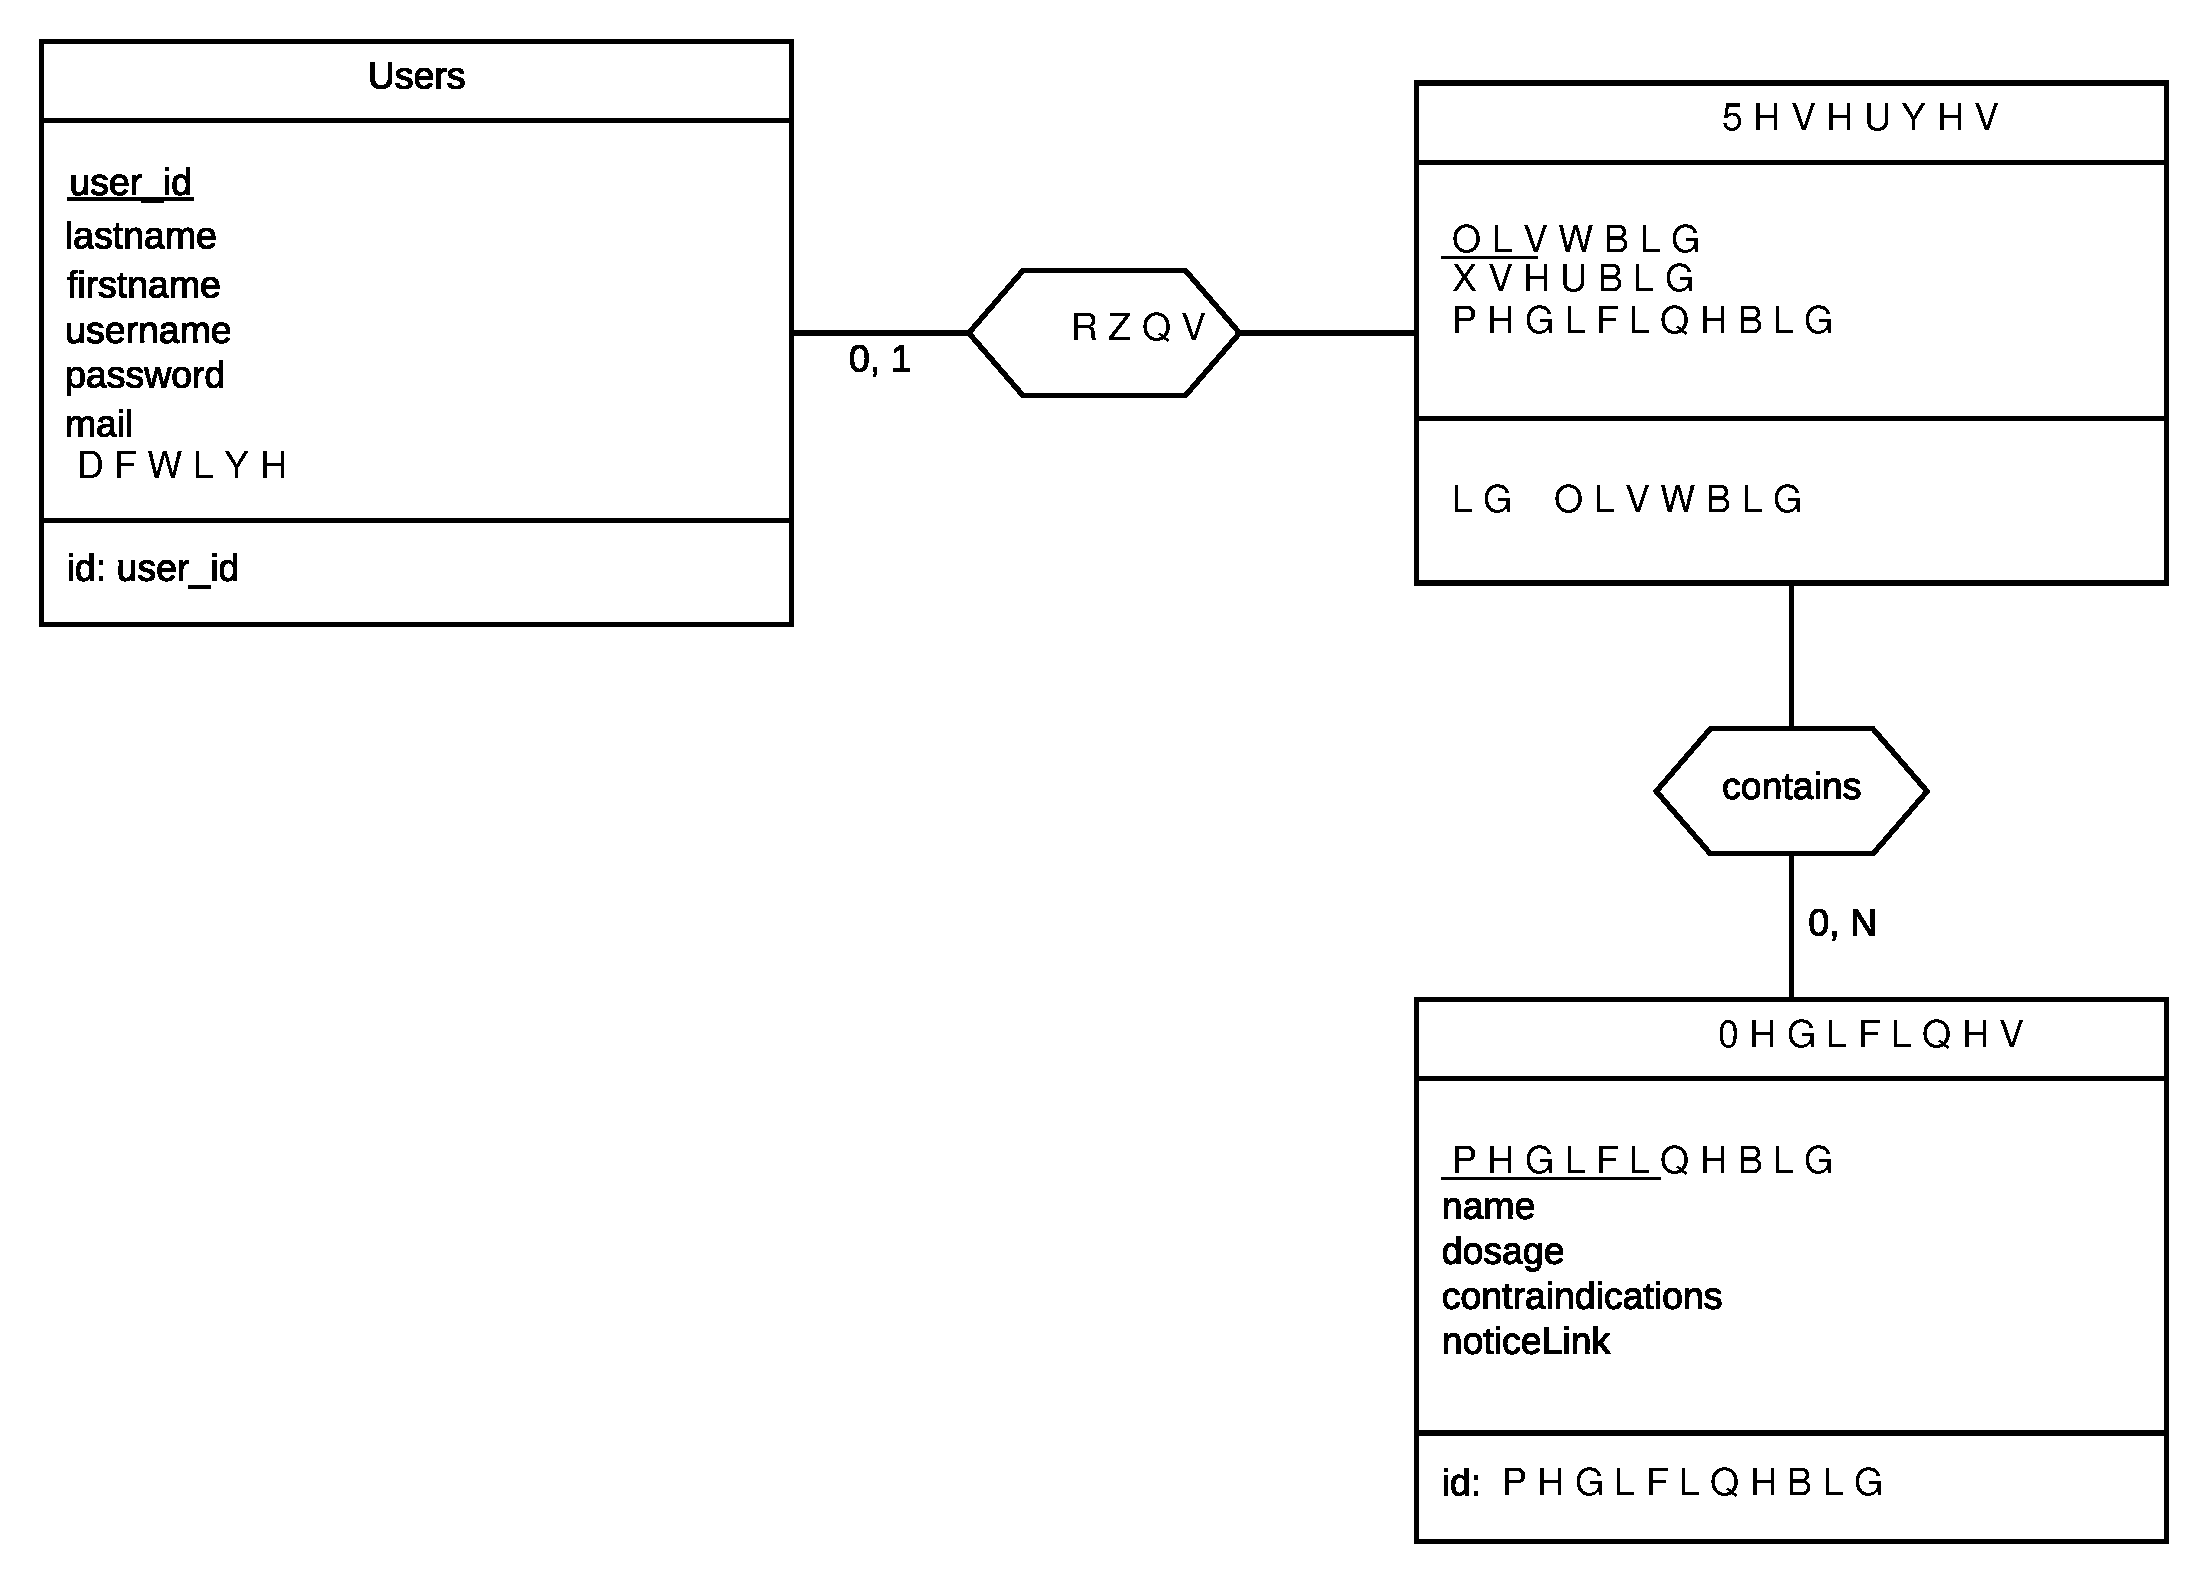
\includegraphics[scale=0.4]
  {textures/images/db/DB.pdf}
  \caption{Schéma conceptuel de la base de données}
  \label{fig:db}
\end{figure}

\newpage

\subsection{Vue détaillée}
\label{sec:vue-details}


\subsubsection{Table Medicines}
\label{sec:table-med}

Cette table contient les informations de chaque médicament.\\

\begin{itemize}
    
    \item[$\bullet$] \textbf{medicine\_id} est l'identifiant du médicament.\\
    Il sert de clé primaire de la table et est auto-incrémenté à partir de 1.
    
    \item[$\bullet$] \textbf{name} est le nom du médicament.\\
    Ce champ, en plus de contenir le médicament, identifie son type: comprimé, comprimé effervescent, gélule, etc.
    
    \item[$\bullet$] \textbf{dosage} contient le ou les différents dosages possibles \textit{(en mg ou en g)}.
    
    \item[$\bullet$] \textbf{contraindications} comprend deux à trois lignes de contre-indications du médicament.
    
    \item[$\bullet$] \textbf{noticeLink} contient l'adresse vers la notice en ligne, à télécharger.
    
\end{itemize}

\textbf{\textit{Remarque : }} l'image représentant le médicament est sauvegardée dans un dossier spécifique et est liée à son identifiant.\\
Elle ne se trouve donc pas dans la base de données.


\subsubsection{Table Reserves}
\label{sec:table-res}

Cette table lie les deux autres: la réserve de médicaments lie chaque utilisateur à ses médicaments.\\

\begin{itemize}

    \item[$\bullet$] \textbf{list\_id} est l'identifiant unique de la réserve.\\
    Il est auto-incrémenté à partir de un et sert de clé primaire.
    
    \item[$\bullet$] \textbf{user\_id} est l'identifiant de l'utilisateur.\\
    C'est une clé étrangère.
    
    \item[$\bullet$] \textbf{medicine\_id} identifie les médicaments.\\
    C'est aussi une clé étrangère.
    
\end{itemize}

\newpage

\subsubsection{Table Users}
\label{sec:table-users}

C'est la table contenant les données de chaque utilisateur ainsi que l'état de leur compte.\\

\begin{itemize}
    
    \item[$\bullet$] \textbf{user\_id} est l'identifiant unique du médicament.\\
    Il sert de clé primaire de la table et est auto-incrémenté à partir de un.
    
    \item[$\bullet$] \textbf{lastname} est le nom de famille de l'utilisateur.
    
    \item[$\bullet$] \textbf{firstname} est le prénom de l'utilisateur.
    
    \item[$\bullet$] \textbf{username} est le nom d'utilisateur unique choisi lors de l'inscription.
    
    \item[$\bullet$] \textbf{password} est le mot de passe de l'utilisateur.\\
    Il a une taille minimale de 4 caractères et est haché \footnote{\url{https://fr.wikipedia.org/wiki/Fonction\_de\_hachage\_cryptographique}} \textit{(et salé)} à l'aide de SHA512.
    
    \item[$\bullet$] \textbf{mail} contient l'adresse mail de l'utilisateur.\\
    Ce champ est unique, vu qu'il sert à la connexion de l'utilisateur.
    
    \item[$\bullet$] \textbf{active} donne l'état du compte de l'utilisateur:
    
    \begin{itemize}
        
        \item \textbf{0} indique que le compte est inactif.\\
        Cela signifie que le compte a été supprimé ou que l'administrateur a banni l'utilisateur.
        
        \item \textbf{1} indique que le compte est actif \textit{(par défaut)}.
        
    \end{itemize}
    
\end{itemize}


%%% Local Variables:
%%% mode: latex
%%% TeX-master: t
%%% End:
\newpage
\section*{Le site}
\addcontentsline{ptc}{section}{Le site}
\label{sec:site}

Voici les différentes pages du site finalisé :

\begin{figure}[!h]
    \centering
    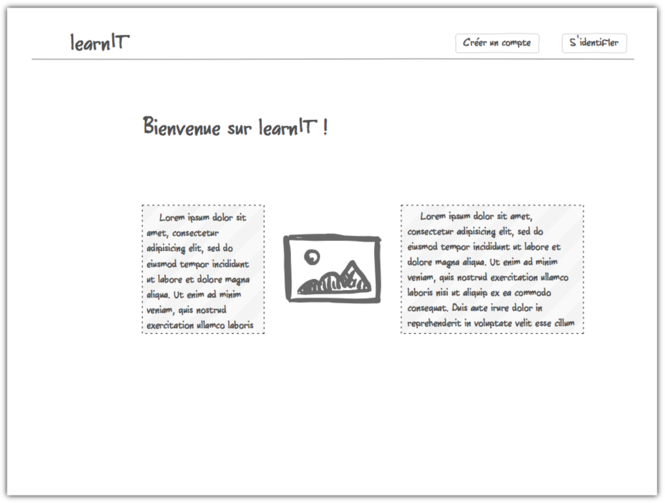
\includegraphics[scale=1]{textures/images/annexes/site/1a-Home.png}
    \caption{La page d'accueil}
\end{figure}
\begin{figure}[!h]
    \centering
    \includegraphics[scale=1]{textures/images/annexes/site/1b-CréerCompte.png}
    \caption{La page d'inscription}
\end{figure}

\newpage

\begin{figure}[!h]
    \centering
    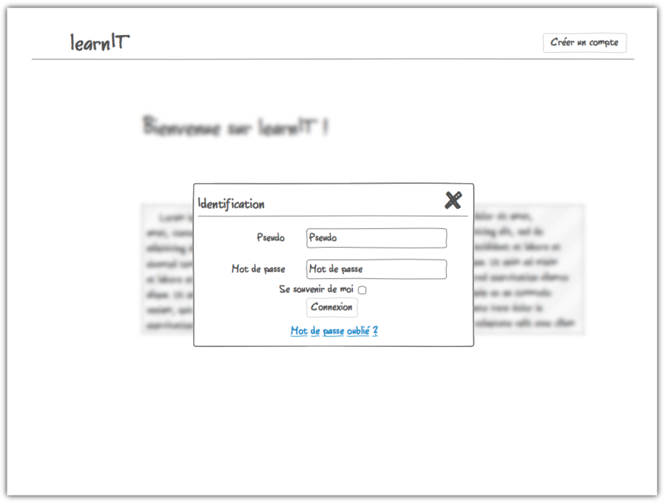
\includegraphics[scale=1]{textures/images/annexes/site/1c-Sidentifier.png}
    \caption{La page de connexion}
\end{figure}
\begin{figure}[!h]
    \centering
    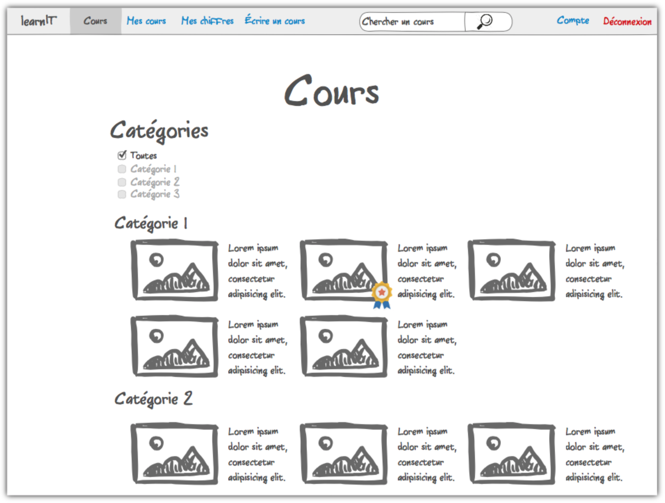
\includegraphics[scale=1]{textures/images/annexes/site/2-Cours.png}
    \caption{La liste des cours}
\end{figure}

\newpage

\begin{figure}[!h]
    \centering
    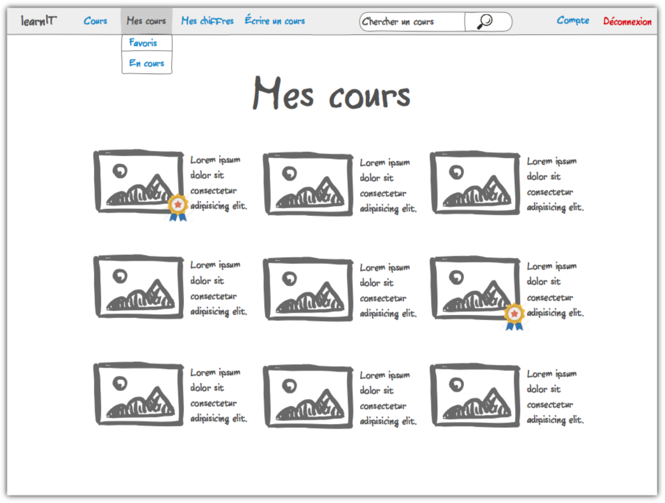
\includegraphics[scale=1]{textures/images/annexes/site/3-MesCours.png}
    \caption{La liste des cours auxquels l'utilisateur est inscrit}
\end{figure}
\begin{figure}[!h]
    \centering
    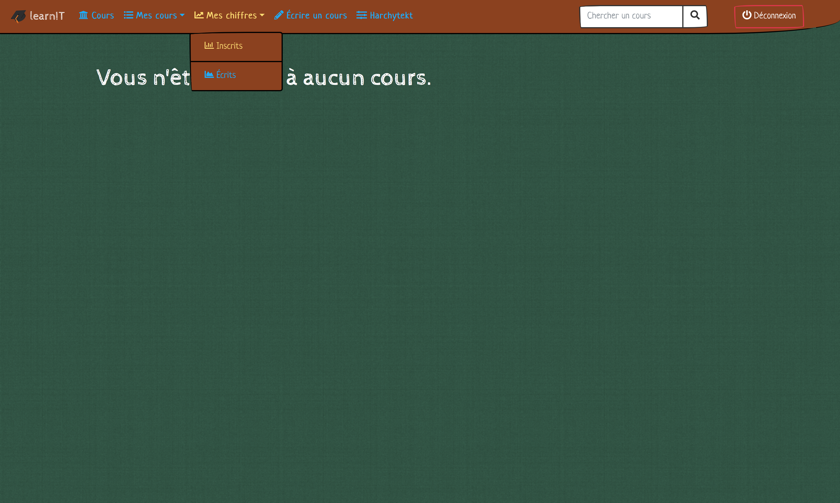
\includegraphics[scale=1]{textures/images/annexes/site/4-MesChiffres(Cours).png}
    \caption{La page des chiffres}
\end{figure}

\newpage

\begin{figure}[!h]
    \centering
    \includegraphics[scale=1]{textures/images/annexes/site/5-ÉcrireCours.png}
    \caption{La page de création d'un cours}
\end{figure}
\begin{figure}[!h]
    \centering
    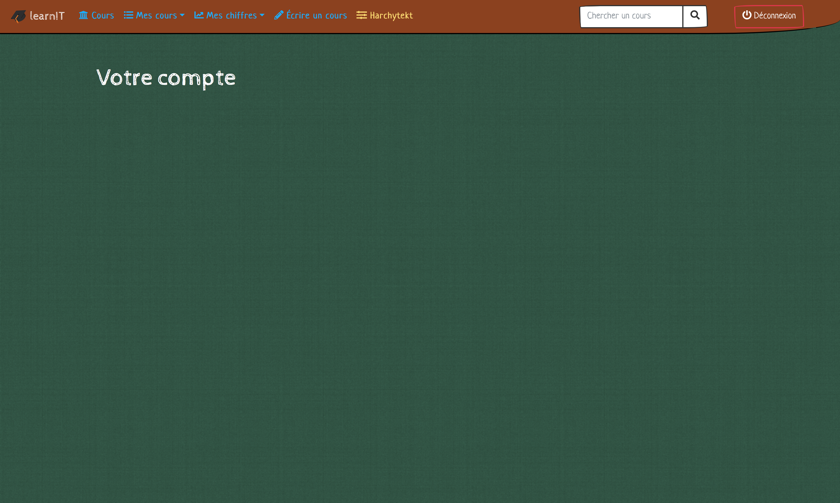
\includegraphics[scale=1]{textures/images/annexes/site/6-Compte(utilisateur).png}
    \caption{La page du compte utilisateur}
\end{figure}
\newpage
\section{Conclusion}
\label{sec:conclusion}


\subsection{Résultat}
\label{sec:resultat}

L'automate trie les boites d'après leur couleur \textit{(argent, cuivre et or)}.\\

Lorsqu'il est à l'arrêt, la lampe \textit{Hors-service} est allumée, et la lampe \textit{En service} est éteinte. \\

L'appui sur le bouton poussoir  \guillemotleft \ \textbf{Start} \guillemotright \ allume la lampe \textit{En service}, éteint la lampe \textit{Hors-service} et met en route le moteur du convoyeur principal.\\
Sauf dans le cas où un défaut moteur a été détecté, ce qui arrêterait \textit{totalement} le fonctionnement de l'automate.\\
Celui-ci devra d'abord être corrigé afin de désactiver l'alarme lumineuse par un acquittement à l'aide du sélecteur à clé \textbf{I16}. Le moteur pourra alors être mis en route.\\

Pour mettre en marche le moteur des convoyeurs d'évacuation, le sélecteur \textbf{I17} doit être enclenché.\\
S'il n'est pas enclenché, un défaut moteur sera levé et affiché par la lampe \textbf{Q1}. Voici les différents cas qui lèveront le défaut :

\begin{itemize}
    
    \item le cas du défaut au moteur principal, c'est le cas le plus simple.\\
    Le moteur se retrouve en surcharge, ce qui enclenche l'arrêt d'urgence.
    
    \item le cas du défaut au moteur des convoyeurs d'évacuation, divisé en différents cas.
    
    \begin{itemize}
    
        \item le cas simple, le moteur est en surcharge, ce qui enclenche l'arrêt d'urgence.
        
        \item le cas de l'encombrement des tapis d’évacuation.\\
        Il est levé lorsqu'une boite est sous le détecteur du tapis d'évacuation, et qu'une autre \textit{(du même type)} se retrouve devant le vérin.\\
        C'est le cas lorsque le moteur des tapis d’évacuation est à l'arrêt.
        
        \item le cas \textit{bonus}, les tapis d'évacuation sont stoppés, mais le moteur principal ne l'est pas.\\
        Lorsqu'une boite est détectée par le dernier détecteur, \textbf{I3}, un défaut est levé.\\
        Sans ce dernier cas, la boite tomberait du tapis.
        
    \end{itemize}
    
\end{itemize}

\newpage

Lorsqu'une boite argentée ou cuivrée est repérée par le détecteur idoine, le moteur principal s'arrête et le vérin place la boite sur le tapis d'évacuation approprié.\\
Le vérin se replace et le moteur principal se relance une fois que la boite est détectée sur son tapis d'évacuation.\\
À ce moment, le compteur qui lui est lié s'incrémente de un.\\

Pour les boites dorées, il n'y a pas de vérin, donc pas d'arrêt du moteur principal.\\
En effet, une fois arrivées au bout du tapis principal, les boites se retrouvent sur le tapis d'évacuation correct s'il est activé.\\
C'est alors le dernier détecteur, \textbf{I3}, qui incrémente le compteur adéquat.\\

Les compteurs sont réinitialisés dans deux cas :

\begin{itemize}
    
    \item premier cas, l'automate est stoppé par le bouton poussoir \guillemotleft \ \textbf{Stop} \guillemotright.
    
    \item second et dernier cas, le sélecteur à clé, \textbf{I18}, est activé afin de réinitialiser les compteurs à la main.
    
\end{itemize}

\newpage
\newpage
\thispagestyle{empty}
\setcounter{page}{0}
\null
\newpage
\end{document}
